\documentclass[12pt,twoside]{scrartcl}
\usepackage[a4paper,top=2cm,left=2cm,right=2cm,bottom=2cm,includefoot,includehead]{geometry}
\usepackage{graphicx}
\usepackage[numbers]{natbib} % Add this line for natbib package
\usepackage{caption}
\usepackage{fancyhdr}
\usepackage{hyperref}
\usepackage{amsmath}
\usepackage{amsfonts}
\usepackage{circuitikz}
\graphicspath{ {figures/} }


\ctikzset{
    resistor = american,
    % inductor = american,
    voltage = raised ,
    voltage dir = old,
    quadpoles/transformer core/inner = 1, %Eliminates the horizontal bars on the transformer
    quadpoles/transformer core/width = 0.8, %Adjusts the width so that the transformers are closer
    diodes/scale = 0.6,
    capacitors/scale = 0.6,
    resistors/scale = 0.6,
    inductors/scale = 0.8,
    % bipoles/label_distance = 4pt,
    % switch/scale = 0.8,
    % bipoles/length = 1cm,
}

%% shifted open voltage 
\tikzset{open shifted/.style={
    open ,open voltage position=legacy, voltage shift=-0.9}
}

\pagestyle{fancy} % Set the page style to fancy
\fancyhf{} % Clear all header and footer fields

% Define the header and footer content for odd and even pages
\fancyhead[CE]{School of Electrical and Computer Engineering}
\fancyhead[CO]{Power Electronics and Renewable Energy Systems} % Left header on even pages, right header on odd pages
% \fancyhead[RE,LO]{Right Header} % Right header on even pages, left header on odd pages
\fancyfoot[LE,RO]{\thepage} % Page number on left footer of even pages and right footer of odd pages
% \fancyfoot[RE,LO]{ELEC3251} % Left footer on odd pages, right footer on even pages

\hypersetup{colorlinks, citecolor=voilet, linkcolor=blue, urlcolor=blue}


\begin{document}
\pagenumbering{arabic}
\setcounter{page}{1}
\begin{titlepage}
    \begin{center}

        
\includegraphics[width=0.2\textwidth]{LOGO_Square.pdf}

        \vspace*{0.4cm}
        School of Electrical and Computer Engineering \\
        University of Newcastle, Australia
        
        \vspace{1cm}
        \huge
        \textbf{\textsf{ELEC3251 \\ }}
        \vspace{0.2cm}
        \huge
        \textbf{\textsf{Assignment 2 \\ }}
        \vspace{1cm}
        \normalsize
        Liam Patey-Dennis \\
        c3349900 \\
        \vspace{2.5cm}
        \large
        \textbf{\textsf{Analysis of Switching Harmonics \\ 
                        and Grid Connected Inverters
                        }}

        
        \vfill    
    \end{center}
\end{titlepage}


\section{PV Voltage and Switching Harmonics}
\subsection{Method}
To determine the correct switching output, a test was performed at the H-bridge output to confirm that both
switching strategies can be achieved. 
This test involved setting a constant sinusoid input at the H-bridge controller.
\begin{figure}[htp]
    \centering
    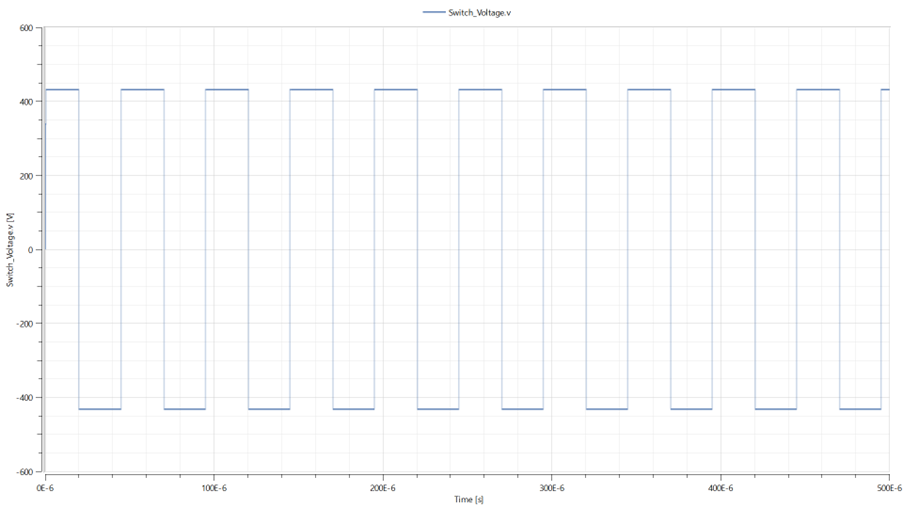
\includegraphics[width=0.7\textwidth]{Bipolar_sw.png}
    \caption{Bipolar Switching Test}
    \label{fig:Bipolar Switching}
\end{figure}
\begin{figure}[htp]
    \centering
    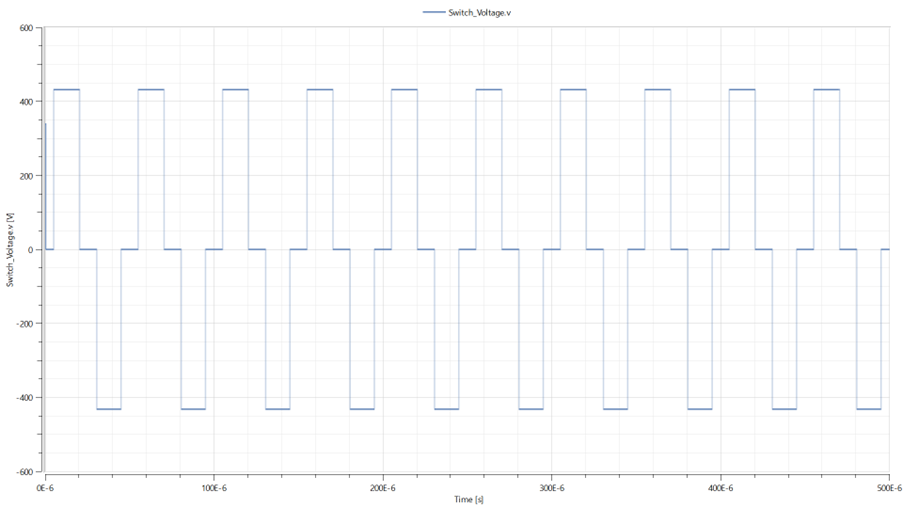
\includegraphics[width=0.7\textwidth]{Unipolar_sw.png}
    \caption{Unipolar Switching Test}
    \label{fig:Unipolar Switching}
\end{figure}
\newpage
\noindent
\begin{figure}[htp]
    \centering
    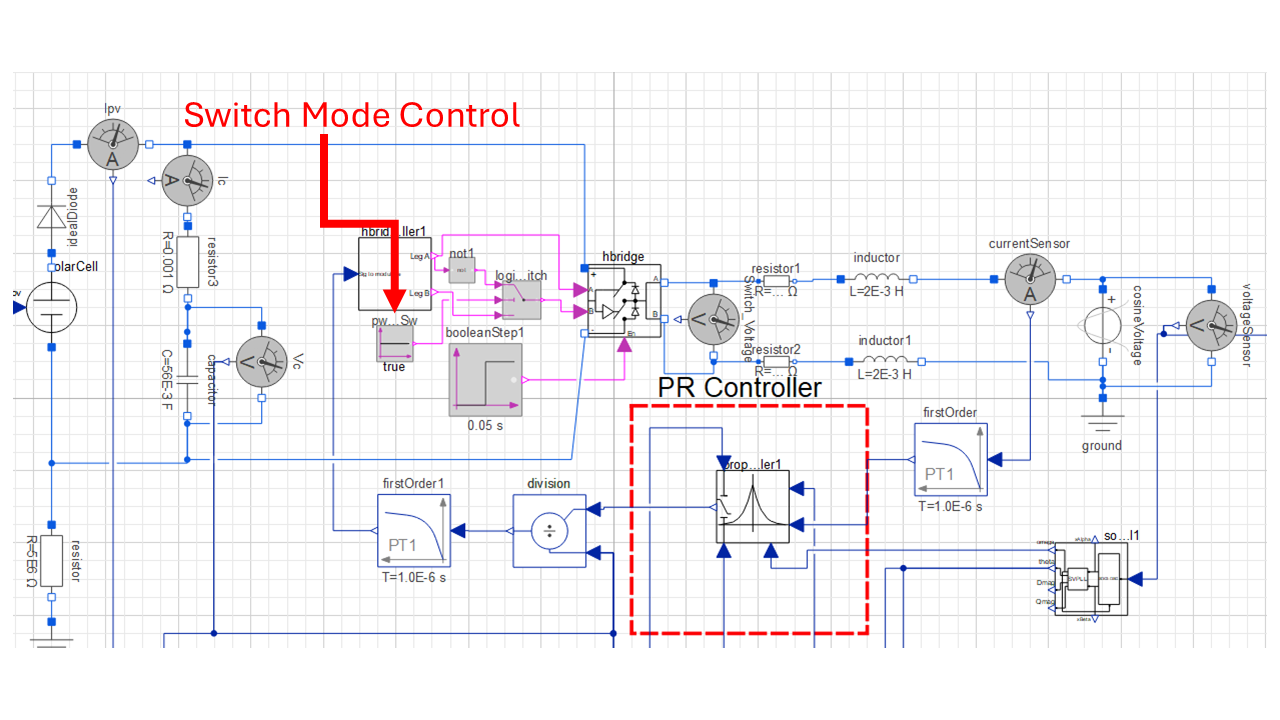
\includegraphics[width=0.7\textwidth]{Set-Up.PNG}
    \caption{How to set bipolar and unipolar switching}
    \label{fig:Set Up}
\end{figure}
The switching frequency was set to 20$\: kHz$. The current sensor, Ic was added to measure current 
through the capacitor. The voltage sensor for the capacitor was named Vc. The simulation was run twice, at 0.2 s and at 10 s. This allows the 
viewing of different frequency components. The numbers of cells in series for the solar cell was 850. The capacitance was set to 56 mF. The some experimentation,
it was found that the input supply was 5kW.
\newpage
\subsection{Results}
\begin{figure}[htp]
    \centering
    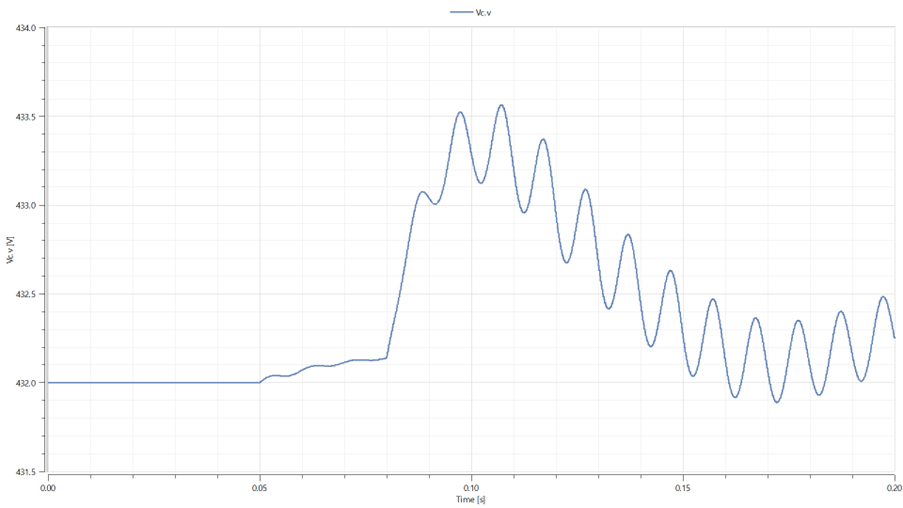
\includegraphics[width=0.75\textwidth]{Bipolar_Vc_0.2.png}
    \caption{Bipolar $V_c$, capacitor voltage (PV to GND), Sim Time = 0.2 s}
    \label{fig:BipolarVc0.2}
\end{figure}
\begin{figure}[htp]
    \centering
    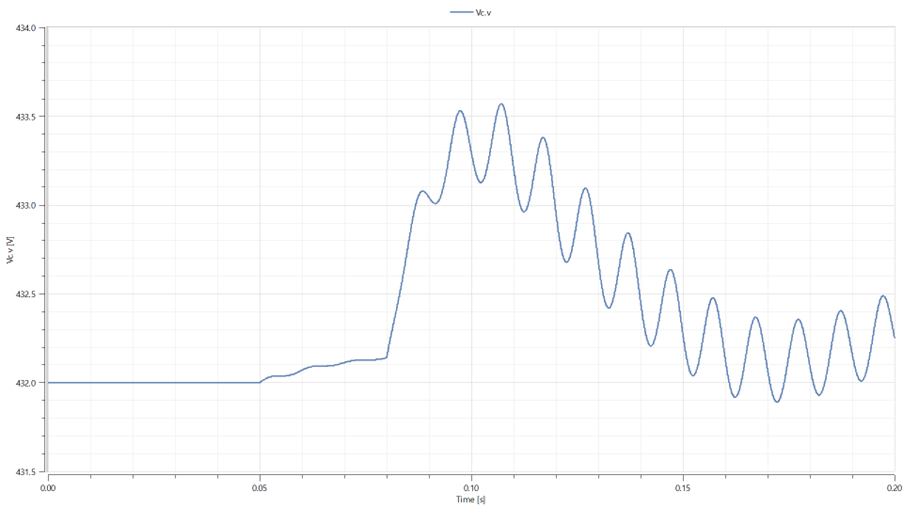
\includegraphics[width=0.75\textwidth]{Unipolar_Vc_0.2.png}
    \caption{Unipolar $V_c$, capacitor voltage (PV to GND), Sim Time = 0.2 s}
    \label{fig:UnipolarVc0.2}
\end{figure}
\begin{figure}[htp]
    \centering
    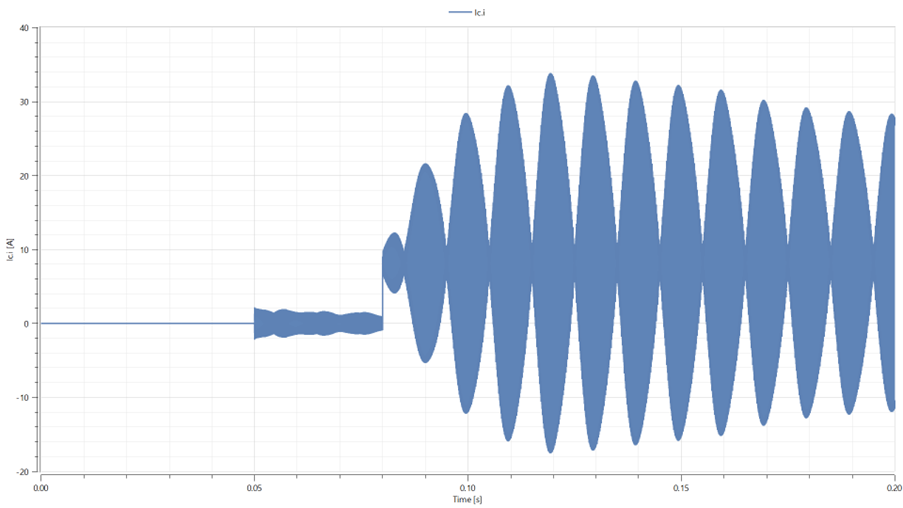
\includegraphics[width=0.8\textwidth]{Bipolar_Ic_0.2.png}
    \caption{Bipolar $I_c$, current through capacitor, Sim Time = 0.2 s}
    \label{fig:BipolarIc0.2}
\end{figure}
\begin{figure}[htp]
    \centering
    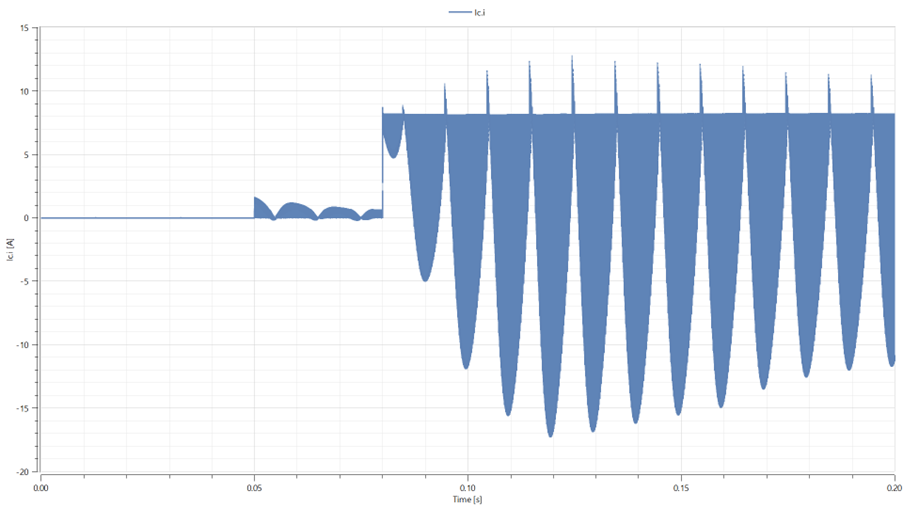
\includegraphics[width=0.8\textwidth]{Unipolar_Ic_0.2.png}
    \caption{Unipolar $I_c$, current through capacitor, Sim Time = 0.2 s}
    \label{fig:UnipolarIc0.2}
\end{figure}
\begin{figure}[htp]
    \centering
    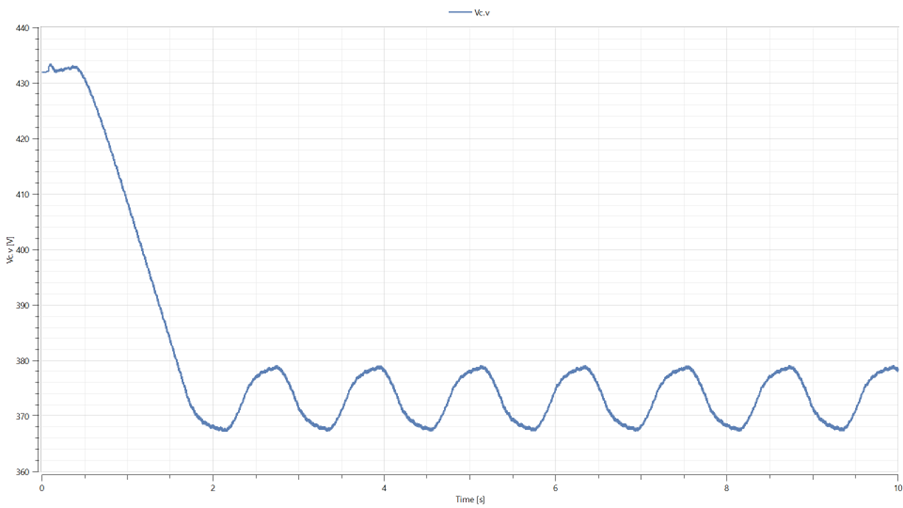
\includegraphics[width=0.75\textwidth]{Bipolar_Vc_10.png}
    \caption{Bipolar $V_c$, capacitor voltage (PV to GND), Sim Time = 10 s}
    \label{fig:BipolarVc10}
\end{figure}
\begin{figure}[htp]
    \centering
    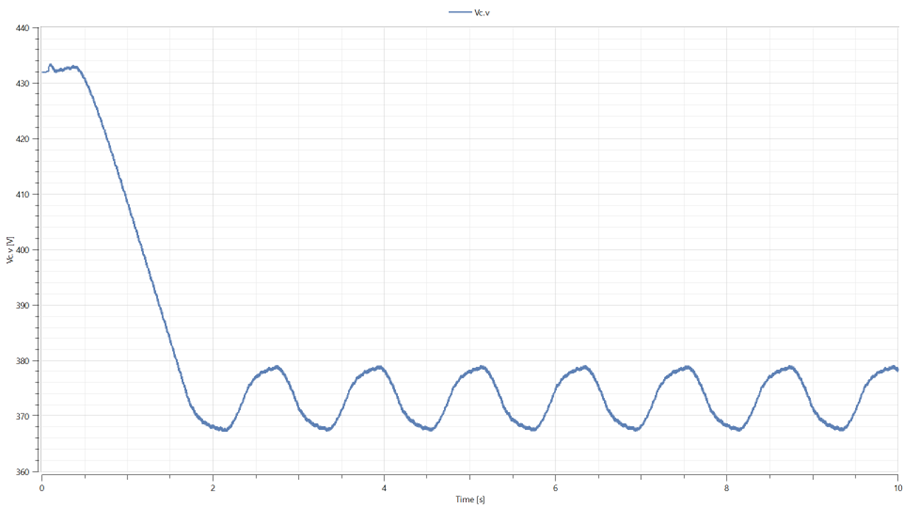
\includegraphics[width=0.75\textwidth]{Unipolar_Vc_10.png}
    \caption{Unipolar $V_c$, capacitor voltage (PV to GND), Sim Time = 10 s}
    \label{fig:UnipolarVc10}
\end{figure}
\begin{figure}[htp]
    \centering
    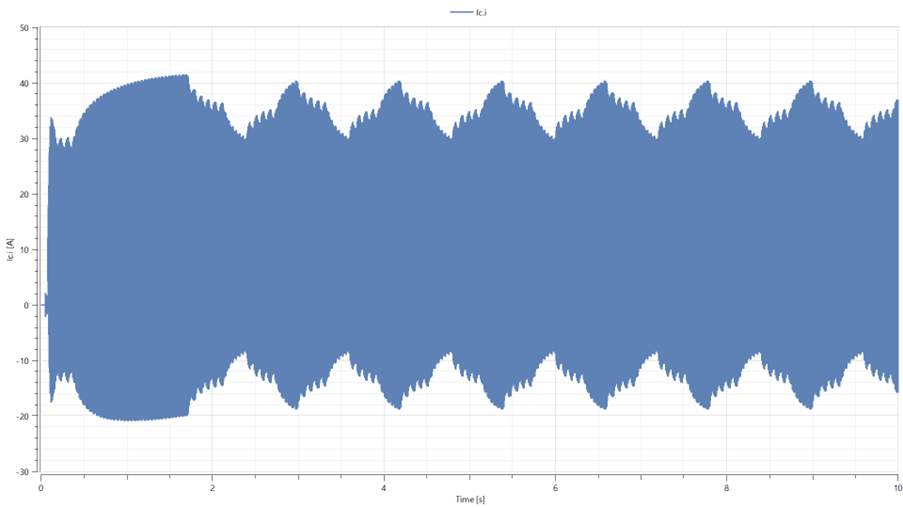
\includegraphics[width=0.8\textwidth]{Bipolar_Ic_10.png}
    \caption{Bipolar $I_c$, current through capacitor, Sim Time = 10 s}
    \label{fig:BipolarIc10}
\end{figure}
\begin{figure}[htp]
    \centering
    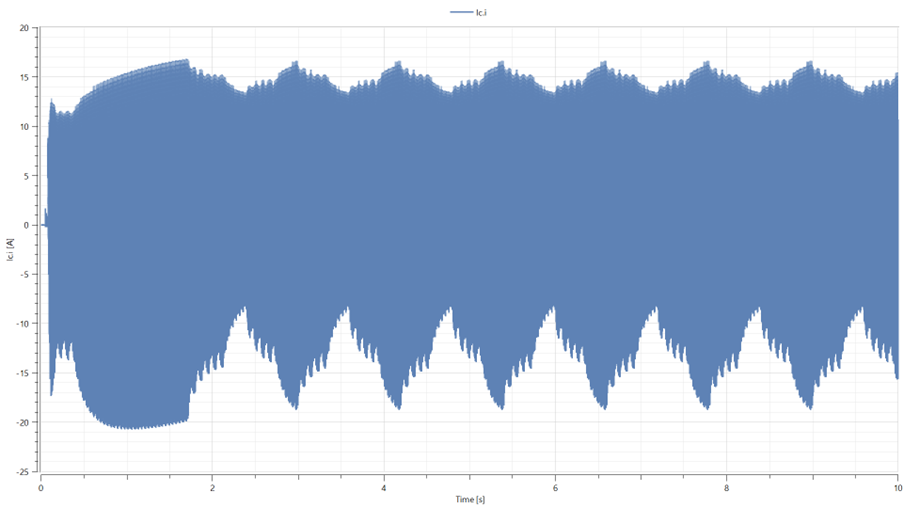
\includegraphics[width=0.8\textwidth]{Unipolar_Ic_10.png}
    \caption{Unipolar $I_c$, current through capacitor, Sim Time = 10 s}
    \label{fig:UnipolarIc10}
\end{figure}
\begin{figure}[htp]
    \centering
    \includegraphics[width=0.8\textwidth]{Bipolar_Vc_ripple.png}
    \caption{Bipolar, voltage ripple $\Delta V_c$ = 0.0054 V, manual zoom}
    \label{fig:BipolarVcripple}
\end{figure}
\begin{figure}[htp]
    \centering
    \includegraphics[width=0.8\textwidth]{Unipolar_Vc_ripple.png}
    \caption{Unipolar, voltage ripple $\Delta V_c$ = 0.0022 V, manual zoom}
    \label{fig:UnipolarVcripple}
\end{figure}
\begin{figure}[htp]
    \centering
    \includegraphics[width=0.8\textwidth]{Bipolar_Ic_rms.png}
    \caption{Bipolar, RMS capacitor current, $I_c$ = 13 $A_{RMS}$ at steady state, Sim Time = 5s}
    \label{fig:BipolarIcRMS}
\end{figure}
\begin{figure}[htp]
    \centering
    \includegraphics[width=0.8\textwidth]{Unipolar_Ic_rms.png}
    \caption{Bipolar, RMS capacitor current, $I_c$ = 10.2 $A_{RMS}$ at steady state, Sim Time = 5s}
    \label{fig:UnipolarIcRMS}
\end{figure}
\newpage
\subsection{Discussion}
Comparing both switching methods, the capacitor voltage (PV) was basically equal, see Figure \ref{fig:BipolarVc0.2}. 
At time 0.05 s the H-bridge starts switching to produce a current. 
For the PV cell, the aim is to obtain 5kW of output power. If power, P is 
\begin{equation}
    P = IV
\end{equation}
and the grid voltage is 240 $V_{RMS}$, then the current must be,
\begin{equation}
    I = \dfrac{P}{V} = \dfrac{5\cdot10^3}{240} = 20.83 \: A_{RMS}
\end{equation}
This makes sense, because later simulations show that 
the supply current at steady state is 29.5$\:A_{p}$. From \ref{fig:UnipolarVc10}, 
a steady state value can be inferred from the PV voltage or capacitor 
voltage, $V_c$. This is 373 $\pm$ 5 V. For its RMS,
\begin{equation}
    373 + \dfrac{5}{\sqrt{2}} = 376.5 \: V_{RMS}
    \label{eq:V_rms}
\end{equation} 
This steady state voltage is the MPP (Maximum Power Point). For this simulation, it happened to be 3.8 kW.
\newline
\newline
\noindent
An analysis of the different $V_c$ plots show many different frequency components.
The first frequency component is the switching frequency, \ref{fig:BipolarVcripple} and \ref{fig:UnipolarVcripple}.
The second frequency component comes from switching trying to match the grid sinusoid, \ref{fig:BipolarIc0.2}. This $f$, is 100 $Hz$. This comes 
from the grid connected voltage. This is 50 $Hz$,
that makes this signal, the second harmonic. The same frequency can 
be seen from the current plots, Figure \ref{fig:BipolarIc0.2}.
There is a distinct difference between the plots, due to the different switching modes, 
see Figure \ref{fig:UnipolarIc0.2}. This is expected, as 
harmonic disturbance should be less under unipolar switching. The greatest piece of 
evidence, can be inferred from the magnitudes of the current plots. 
As the magnitude of the harmonics is from 40 to -20
for bipolar and from 15 to -20 for unipolar. This can be proved by 
calculating and plotting rms capacitor current which is performed below. The last
frequency component was at the steady state, \ref{fig:BipolarVc10}. This frequency component 
is harmonic distortion. We can confirm this by checking for a common denominator as this means its an harmonic multiple. The period, is about 1.2 s which 
was estimated by counting periods within a 2-8 s window. For the common denominator information that matters,
\begin{equation} 
    \hspace{6cm} \dfrac{T_{max}}{a \cdot T_{small}} = \mathbb{N} \hspace{3cm} a = 1,3,5,7,11 ...
\end{equation}
The answer must be a postive integer, it is denoted as a natural number. 
If it is not, that means the prime number max is known. For the 100 $Hz$ frequency component, $a_{max} = 5$,
\begin{equation}
    \dfrac{1.2}{5 \cdot 0.01} = 24 \tag*{}
\end{equation}
For the switching frequency $f_s$, the 20 $kHz$ component, $a_{max} = 5$ as well,
\begin{equation}
    \dfrac{1.2}{5 \cdot 5 \cdot 10^{-5}} = 4800 \tag*{}
\end{equation}
This is expected as the 3rd and 5th harmonics cause the most harmonic 
noise within a single phase system. This 
means that by removing the 3rd and 
5th harmonic, it would remove the majority of the harmonic disturbance at the output.
\newline
\newline
\noindent
The frequency components can be added together to estimate the capacitor current using the capacitor equation,
\begin{equation}
    i_{c} = C\dfrac{dV}{dt}
\end{equation}
To add all the frequency components together, the capacitor equation is expanded like this,
\begin{equation}
    i_c = C\left(\dfrac{dV_1}{dt} + \dfrac{dV_2}{dt} + \dfrac{dV_3}{dt}\right)
\end{equation}
which to discrete,
\begin{equation}
    i_c = C\left(\dfrac{\Delta V_1}{T_1} + \dfrac{\Delta V_2}{0.5T_2} + \dfrac{\Delta V_3}{0.5T_3}\right)
    \label{eq:current_eq}
\end{equation}
Using \ref{eq:current_eq}, Estimates of the period and $\Delta V_c$ for each component from plots \ref{fig:BipolarVcripple}, \ref{fig:BipolarVc0.2}, \ref{fig:BipolarVc10} for bipolar leads to this,
\begin{equation}
    i_c = 56\cdot 10^{-3}\left(0.0054\cdot 20000 + \dfrac{0.5}{0.5 \cdot 0.01} + \dfrac{10}{0.5 \cdot 1.2}\right) = 12.58 \: A_{RMS} \tag*{}
\end{equation}
This can be confirmed by plotting the RMS $i_c$ current, \ref{fig:BipolarIcRMS}. This is set by connecting an RMS block to the current sensor,
then setting the RMS block to frequency 1/1.2 $Hz$. The simulated RMS current is 13 A. This makes an error 3.34\%.
\\
\\
\noindent
For the unipolar simulation, information from plots \ref{fig:UnipolarVcripple}, \ref{fig:UnipolarVc0.2}, \ref{fig:UnipolarVc10}
\begin{equation}
    i_c = 56\cdot 10^{-3}\left(0.0022\cdot 20000 + \dfrac{0.5}{0.5 \cdot 0.01} + \dfrac{10}{0.5 \cdot 1.2}\right) = 8.98 \: A_{RMS} \tag*{}
\end{equation}
Checking against the simulation, \ref{fig:UnipolarIcRMS}, RMS capacitor current is 10.2 A. This makes an error of of 13.59\%. 
This is to be expected, as this was an estimate. Technically,
\begin{equation}
    \dfrac{\Delta V_3}{0.5T_3} = \dfrac{\Delta V_{3rd}}{0.5T_{3rd}} + \dfrac{\Delta V_{5th}}{0.5T_{5th}}
\end{equation}
This is true for the switching and grid noise components. If more time was given, an FFT would have been simulated. 
\newpage
\section{Grid Connected Inverters}
\subsection{Method}
\begin{figure}[htp]
    \centering
    \includegraphics[width=0.7\textwidth]{Set-Up2.PNG}
    \caption{Set Up to confirm grid connected inverter control}
    \label{fig:Real-Set-Up}
\end{figure}
\noindent
This simulation tests the control systems ability to perform output 
disturbance rejection. If the load chabnges,
how does the system react. This simulation changes the real part 
of the load from 5 to 2.5 $\Omega$ at 0.25s. The control system starts at
0.005 s. The H-bridge starting switching at 0.05 s. To reach steady 
state earlier, the capacitor initialisation voltage was set to 360 V.
\newpage
\subsection{Results}
\begin{figure}[htp]
    \centering
    \includegraphics[width=0.75\textwidth]{I_delivered_0.8.png}
    \caption{Current delivered from inverter}
    \label{fig:deliveredcurrent}
\end{figure}
\begin{figure}[htp]
    \centering
    \includegraphics[width=0.75\textwidth]{Grid_current_0.8.png}
    \caption{Current delivered to load from grid voltage source}
    \label{fig:gridcurrent}
\end{figure}
\begin{figure}[htp]
    \centering
    \includegraphics[width=0.8\textwidth]{Grid_voltage_0.8.png}
    \caption{Grid Voltage}
    \label{fig:gridvoltage}
\end{figure}
\newpage
\subsection{Discussion}


\newpage
\bibliographystyle{IEEEtranN}
\bibliography{references}

\end{document}
